% shared-layout-id: 325dc42888015bd31db34f55c04dbb58d6a73904ec7ce0b73c3db88e8e769f67
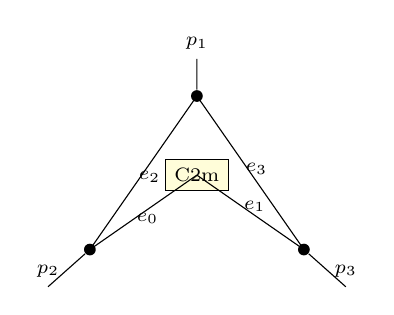
\begin{tikzpicture}[scale=.65,every node/.style={font=\scriptsize}]
\node[rectangle,draw,fill=yellow!15] (v0) at (3.27272727,2.63636364) {C2m};
\node[circle,fill,inner sep=1.5pt] (v1) at (3.27272727,4.18181818) {};
\node[circle,fill,inner sep=1.5pt] (v2) at (1.18181818,1.18181818) {};
\node[circle,fill,inner sep=1.5pt] (v3) at (5.36363636,1.18181818) {};
\draw[black] (3.27272727,2.63636364) .. controls (2.57575758,2.15151515) and (1.87878788,1.66666667) .. (1.18181818,1.18181818);
\node at (2.31033665,1.78968652) {$e_{0}$};
\draw[black] (3.27272727,2.63636364) .. controls (3.96969697,2.15151515) and (4.66666667,1.66666667) .. (5.36363636,1.18181818);
\node at (4.40124574,2.02849530) {$e_{1}$};
\draw[black] (3.27272727,4.18181818) .. controls (2.57575758,3.18181818) and (1.87878788,2.18181818) .. (1.18181818,1.18181818);
\node at (2.34660337,2.59864834) {$e_{2}$};
\draw[black] (3.27272727,4.18181818) .. controls (3.96969697,3.18181818) and (4.66666667,2.18181818) .. (5.36363636,1.18181818);
\node at (4.43751246,2.76498802) {$e_{3}$};
\draw (v1) -- (3.27272727,4.90909091) node[above] {$p_{1}$};
\draw (v2) -- (0.36363636,0.45454545) node[above] {$p_{2}$};
\draw (v3) -- (6.18181818,0.45454545) node[above] {$p_{3}$};
\end{tikzpicture}